Agora estamos trabalhando com modularização...

\begin{figure}[h]
	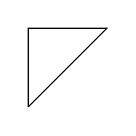
\begin{tikzpicture}
		\draw (0,0) -- (1,1)-- (0,1) -- (0,0);
	\end{tikzpicture}
	\caption[fig:reta]{Primeiro triângulo}
\end{figure}

\begin{figure}[h]
	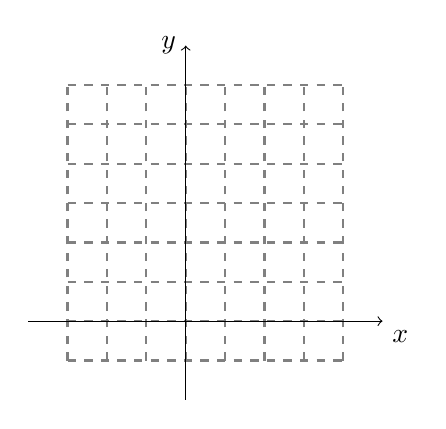
\begin{tikzpicture}[domain=0:4]
		\draw[thick,color=gray,step=.5cm,
		dashed] (-0.5,-.5) grid (3,3);
		\draw[->] (-1,0) -- (3.5,0)
		node[below right] {$x$};
		\draw[->] (1,-1) -- (1,3.5)
		node[left] {$y$};	
	\end{tikzpicture}
	
	\caption[pic:pic2d]{Plano cartesiano}
\end{figure}



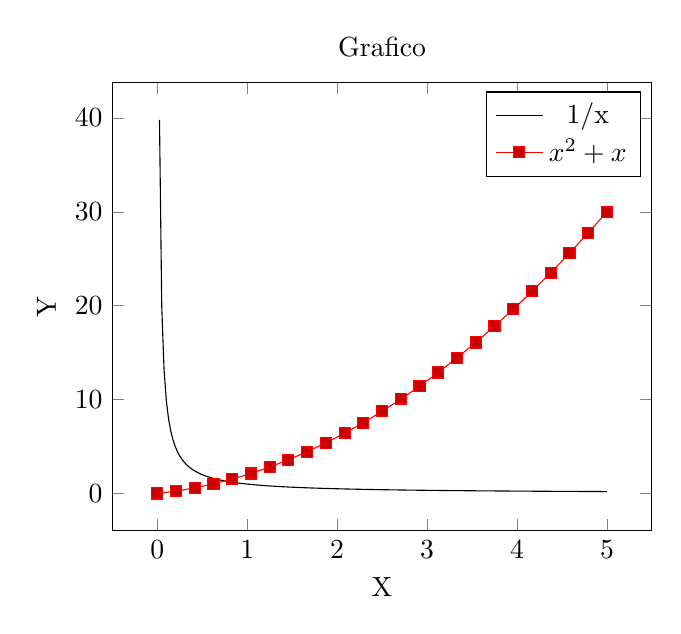
\begin{tikzpicture}[domain=0:5]
	\begin{axis}[xlabel=X,ylabel=Y, title=Grafico]% função
		\addplot[samples=200] {1/x}; %Foco na taxa de amostragem
		\addplot {x^2+x};
		
		\legend{ 1/x, $x^2+x$}
	\end{axis}
\end{tikzpicture}

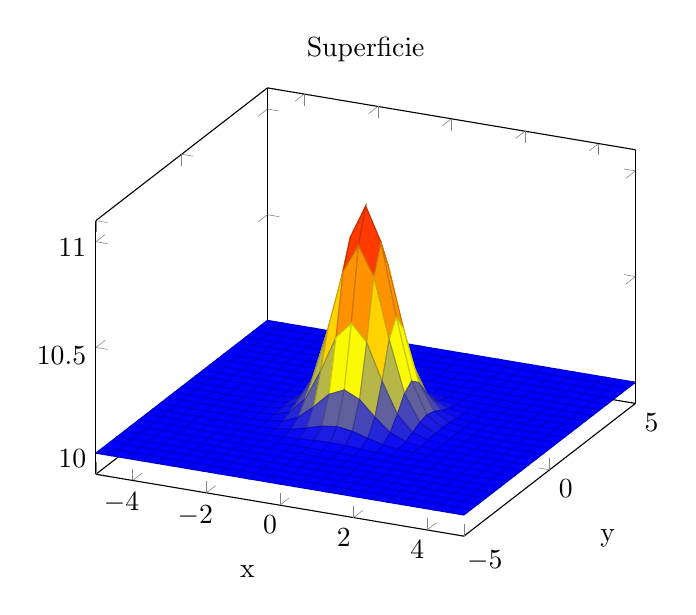
\begin{tikzpicture}
	\begin{axis}[xlabel=x, ylabel=y, title=Superficie ]
%		\addplot3[surf] { (x*y)/(x^2+y^2) }; %Parametro opcional surf 
		\addplot3[surf] {exp(-x^2-y^2)+10};
	\end{axis}
\end{tikzpicture}

Preciso fazer tudo na mão?

	\definecolor{wrwrwr}{rgb}{0.3803921568627451,0.3803921568627451,0.3803921568627451}
	\definecolor{rvwvcq}{rgb}{0.08235294117647059,0.396078431372549,0.7529411764705882}
	\begin{tikzpicture}[line cap=round,line join=round,>=triangle 45,x=1cm,y=1cm]
		\clip(-14.73,-9.17) rectangle (14.73,9.17);
		\fill[line width=2pt,color=rvwvcq,fill=rvwvcq,fill opacity=0.10000000149011612] (-12.77,8.03) -- (-12.97,5.31) -- (-9.35,5.35) -- cycle;
		\draw [line width=2pt,color=rvwvcq] (-12.77,8.03)-- (-12.97,5.31);
		\draw [line width=2pt,color=rvwvcq] (-12.97,5.31)-- (-9.35,5.35);
		\draw [line width=2pt,color=rvwvcq] (-9.35,5.35)-- (-12.77,8.03);
		\draw [line width=2pt,color=wrwrwr] (-11.47,1.75) circle (1.7418381095842403cm);
		\draw [line width=2pt,color=wrwrwr] (-10.49,3.19) circle (1.7801123560045298cm);
		\draw [line width=2pt,color=wrwrwr] (-9.736764083270547,1.5771033344480134) circle (1.5427899996524417cm);
		\begin{scriptsize}
		\draw [fill=rvwvcq] (-12.77,8.03) circle (2.5pt);
		\draw [fill=rvwvcq] (-12.97,5.31) circle (2.5pt);
		\draw [fill=rvwvcq] (-9.35,5.35) circle (2.5pt);
		\draw [fill=rvwvcq] (-11.47,1.75) circle (2.5pt);
		\draw [fill=rvwvcq] (-10.49,3.19) circle (2.5pt);
		\draw [fill=rvwvcq] (-8.71,3.21) circle (2.5pt);
		\draw [fill=wrwrwr] (-9.736764083270547,1.5771033344480134) circle (2pt);
		\draw [fill=rvwvcq] (-8.95,0.25) circle (2.5pt);
	\end{scriptsize}
\end{tikzpicture}

Segundo \cite{art:dilma}, $25\%$ de $30\%$ não é $25\%$ de...
Para \citealp{art:vampirao}, tudo é uma questão de próclise e mesóclise:
\begin{quotation}
	Fazê-lo-ei-lo-lhe e dá-le-ei-lo-lha um \textit{impeachment}.
\end{quotation}





